%!TEX root = ../thesis.tex

\section{ルールベース制御器}

  学習フェーズで用いるルールベース制御器は,前節で述べた2DLiDARの反射強度を利用している.ルールベース制御器の出力は,ロボットのヨ―方向の角速度$\omega$の1つとし,角速度$\omega$が0 \,[rad/s] となるようにロボットを制御する.角速度$\omega$は,以下の式\eqref{eq:angular_velocity}で表され,角度に応じた角速度$\omega$が式\eqref{eq:inequality}の範囲で出力される.

  \begin{equation}
    \omega[\text{rad/s}] = \frac{1}{\theta_{\text{max}}} \times \theta
    \label{eq:angular_velocity}
    \end{equation}

  \begin{equation}
    1 \geq \omega \geq -1
    \label{eq:inequality}
    \end{equation}

  ルールベース制御器からの出力を\tabref{tab:output_from_rule-based_controllers}に示す.ここでは,わかりやすくするために行動を左旋回,直進,右旋回の3つに分解しているが,実際に出力される行動はロボットのヨ―方向の角速度$\omega$の1つということに注意する.

  \begin{table}[h]
    \caption{Output from rule-based controllers}
    \label{tab:output_from_rule-based_controllers}
    \begin{tabular}{|c|c|c|c|}
    \hline
    Action & Control rule {[}rad{]} & Linear velocity {[}m/s{]} & Angular velocity {[}rad/s{]} \\ 
    \hline
    Turn Left & $\text{angle\_max} \geq \theta > 0$ & 0.2 & $1 \geq \omega > 0$ \\ 
    \hline
    Forward & $0$ & 0.2 & $0$ \\ 
    \hline
    Turn Right & $0 < \theta \leq \text{angle\_min}$ & 0.2 & $0 > \omega \geq -1$ \\ 
    \hline
    \end{tabular}
    \end{table}

\newpage

  ルールベース制御器によるロボットの行動を\figref{Fig:RobotGuidance_learning_turn_left}と\figref{Fig:RobotGuidance_learning_turn_right}に示す.これは,RVizで部分的に可視化したもので,右足に装着した再帰反射テープに反応し,最大反射強度として周辺の色(黄色)とは違う色(紫色)で表示している.
  
  \figref{Fig:RobotGuidance_learning_turn_left}の(a)は,2DLiDARの左前方にいる人(再帰反射テープ)を検出し,その角度に応じた角速度$\omega$の値が出力され,左旋回する.その結果,(b)のように角速度$\omega$はほぼ0 \,[rad/s]に近づき,直進する.

  \figref{Fig:RobotGuidance_learning_turn_right}の(a)は,2DLiDARの右前方にいる人(再帰反射テープ)を検出し,その角度に応じた角速度$\omega$の値が出力され,右旋回する.その結果,(b)のように角速度$\omega$はほぼ0 \,[rad/s]に近づき,直進する.

\begin{figure}[h]
  \centering
  \begin{minipage}[c]{65mm} 
      \centering
      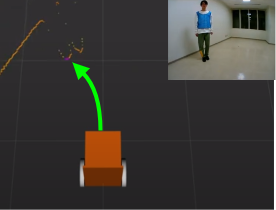
\includegraphics[height=40mm]{images/RobotGuidance_learning_turn_left_(a).png}
      \subcaption{Turn left}
  \end{minipage}
  \begin{minipage}[c]{65mm} 
      \centering
      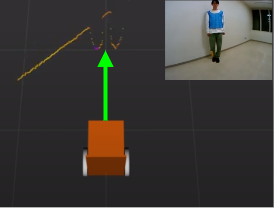
\includegraphics[height=40mm]{images/RobotGuidance_learning_turn_left_(b).png}
      \subcaption{Forward}
  \end{minipage}
  \caption{Turn left toward the retroreflective tape}
  \label{Fig:RobotGuidance_learning_turn_left}
\end{figure}

\begin{figure}[h]
  \centering
  \begin{minipage}[c]{65mm} 
      \centering
      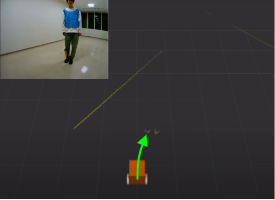
\includegraphics[height=40mm]{images/RobotGuidance_learning_turn_right_(a).png}
      \subcaption{Turn right}
  \end{minipage}
  \begin{minipage}[c]{65mm} 
      \centering
      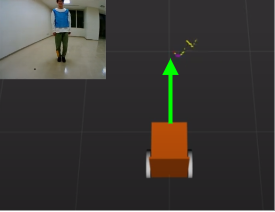
\includegraphics[height=40mm]{images/RobotGuidance_learning_turn_right_(b).png}
      \subcaption{Forward}
  \end{minipage}
  \caption{Turn right toward the retroreflective tape}
  \label{Fig:RobotGuidance_learning_turn_right}
\end{figure}

\newpage
